\documentclass{article}
\usepackage[top=.5in, bottom=.5in, left=.9in, right=.9in]{geometry}
\usepackage[latin1]{inputenc}
\usepackage{enumerate}
\usepackage{hyperref}
\usepackage{graphics}
\usepackage{graphicx}
\usepackage{caption}
\usepackage{subcaption}
\usepackage{tabularx}
\usepackage{amsmath}
\usepackage{amssymb}
\usepackage{siunitx}
\usepackage{mathtools}

\newcommand{\obar}[1]{\ensuremath{\overline{ #1 }}}
\newcommand{\iid}{\ensuremath{\stackrel{\textrm{iid}}{\sim}}}

\usepackage{xcolor}
\definecolor{darkgreen}{rgb}{0,0.25,0}
\newcommand{\soln}{{\color{red}\textbf{Solution:~}\color{black}}}


\usepackage[formats]{listings}
\lstdefineformat{R}{~={\( \sim \)}}
\lstset{% general command to set parameter(s)
basicstyle=\small\ttfamily, % print whole listing small
keywordstyle=\bfseries\rmfamily,
keepspaces=true,
% underlined bold black keywords
commentstyle=\color{darkgreen}, % white comments
stringstyle=\ttfamily, % typewriter type for strings
showstringspaces=false,
numbers=left, numberstyle=\tiny, stepnumber=1, numbersep=5pt, %
frame=shadowbox,
rulesepcolor=\color{black},
,columns=fullflexible,format=R
} %
\renewcommand{\ttdefault}{cmtt}
% enumerate is numbered \begin{enumerate}[(I)] is cap roman in parens
% itemize is bulleted \begin{itemize}
% subfigures:
% \begin{subfigure}[b]{0.5\textwidth} \includegraphics{asdf.jpg} \caption{} \label{subfig:asdf} \end{subfigure}
\hypersetup{colorlinks=true, urlcolor=blue, linkcolor=blue, citecolor=red}


\graphicspath{ {C:/Users/Evan/Desktop/} }
\title{\vspace{-6ex}HW 5\vspace{-2ex}}
\author{Evan Ott \\ UT EID: eao466\vspace{-2ex}}
%\date{DATE}
\setcounter{secnumdepth}{0}
\usepackage[parfill]{parskip}



\begin{document}
\maketitle

\section{Penalized likelihood and soft thresholding}
\subsection{(A)}
First, show that $S_\lambda(y)=\arg\min_\theta \frac{1}{2}(y-\theta)^2+\lambda|\theta|$ has the negative log-likelihood
of a Gaussian distribution with mean $\theta$ and variance 1 as its quadratic term:
\begin{align*}
L(\theta | y) &= \frac{1}{\sqrt{2\pi\cdot 1}}\exp\left(-\frac{(y-\theta)^2}{2\cdot 1}\right)\\
\log L(\theta | y) &= \log\left[\frac{1}{\sqrt{2\pi}}\right]  -\frac{(y-\theta)^2}{2} = c - \frac{(y-\theta)^2}{2}
\end{align*}
So the negative log-likelihood is $\frac{(y-\theta)^2}{2} + c'$ for some $c'\in\mathbb{R}$ that does depends on neither $y$ nor $\theta$, which is exactly the quadratic term in $S_\lambda(y)$.

Now, let's prove the value 
\begin{align*}
S_\lambda(y)&=\arg\min_\theta \frac{1}{2}(y-\theta)^2+\lambda|\theta|\\
\theta > 0:~~ S_\lambda(y)&=\arg\min_\theta \frac{1}{2}(\theta-y)^2+\lambda\theta\\
\Rightarrow~~ 0&=\hat{\theta} - y + \lambda\\
S_\lambda(y)&=\hat{\theta}=y-\lambda\\
\theta < 0:~~ S_\lambda(y)&=\arg\min_\theta \frac{1}{2}(\theta-y)^2-\lambda\theta\\
\Rightarrow~~ 0&=\hat{\theta} - y - \lambda\\
S_\lambda(y)&=\hat{\theta}=y+\lambda\\
\theta = 0:~~ S_\lambda(y)&=0\\
\end{align*}
So, we can now look at the $\arg\min$ as selecting one of those three values of $\hat{\theta}$, depending
on which one has the smallest value of the objective function $f(\hat{\theta})=\frac{1}{2}(y-\hat{\theta})^2+\lambda|\hat{\theta}|$:
\begin{align*}
\theta > 0: ~~ f(\hat{\theta})&=\frac{1}{2}(y-[y-\lambda])^2+\lambda|y-\lambda|\\
&= \frac{\lambda^2}{2} + \lambda|y-\lambda|\\
\theta < 0: ~~f(\hat{\theta})&=\frac{1}{2}(y - [y+\lambda])^2+\lambda|y+\lambda|\\
&= \frac{\lambda^2}{2} + \lambda|y + \lambda|\\
\theta = 0: ~~f(\hat{\theta}) &= \frac{1}{2}(y-0)^2+\lambda|0|\\
&=\frac{y^2}{2}
\end{align*}
Because the second term is a penalty, we can assume $\lambda\geq0$, whereas $y\in\mathbb{R}$. Thus, if $|y| \leq \lambda$, $\hat{\theta}=0$ produces the smallest value of the objective function ($\hat{\theta}\neq0$ has a quadratic term that's larger and adds a non-negative value to that). So $|y|-\lambda\leq0$ produces $S_\lambda(y)=0$ (in particular, $S_\lambda(y)=0$).

Now, if $|y|>\lambda$ we must decide if $\hat{\theta}>0$ or $\hat{\theta}<0$. The quadratic terms are identical, as
is the multiplier of the absolute value term, so the absolute value term is all we need to consider.
Because $\lambda\geq0$, if $y>0$ then $|y-\lambda|<|y+\lambda|$, so $S_\lambda(y)=y-\lambda=|y|-\lambda$. Similarly, if $y<0$ then $|y-\lambda|>|y+\lambda|$ so $S_\lambda(y)=y+\lambda=-|y|+\lambda$. Therefore,

\begin{align*}
S_\lambda(y)&=\left\{
\begin{array}{cc}
0 & y = 0\\
0 & |y| \leq \lambda \wedge y\neq 0 \\
|y|-\lambda & y > 0 \wedge |y| > \lambda\\
-(|y|-\lambda) & y < 0 \wedge |y| > \lambda
\end{array}
\right.=\textrm{sign}(y)(|y|-\lambda)_+
\end{align*}

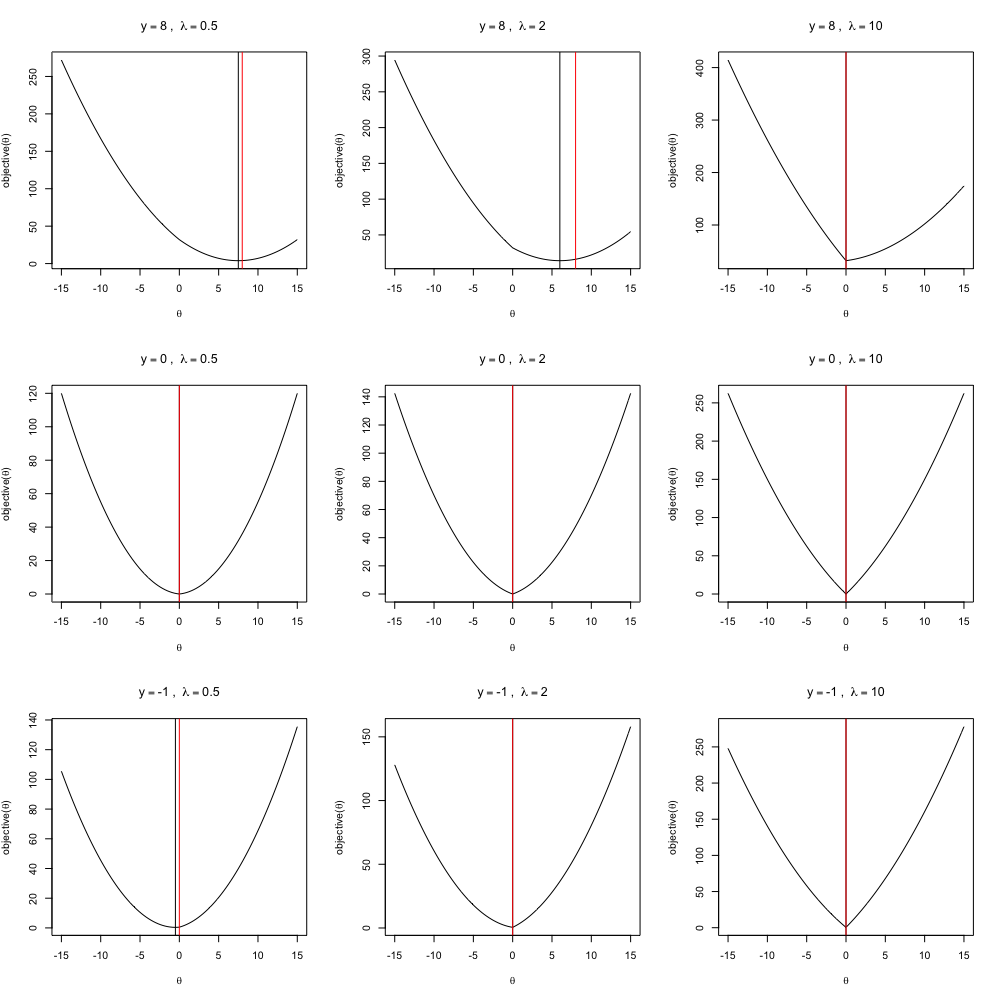
\includegraphics[scale=0.5]{soft_threshold.png}

\subsubsection{Notes from class}
Subdifferential calculus handles things like $|x|$ by allowing more generality. If $f(x)$ has a gradient at $x_0$, then
the only subgradient is the gradient, so the subdifferential is $\{ \nabla f(x_0) \}$. If it doesn't have a gradient there (there's some sort of cusp), then we want $f(x) \geq f(x_0) + g\cdot (x - x_0)$ for all $x$ (this restriction is harsh, and
pretty much only works for convex functions). For example, if $f(x)=|x|$,
then at $x_0=0$ $g=0.5$ would satisfy this (by being below $|x|$ on either side of $x_0$). In this case, any $g\in[-1,1]$
is a subgradient and $[-1,1]$ is the subdifferential.

Theorem. Let $\partial f(x_0)$ be the subdifferential at a given $x_0$. If $f$ is convex, then we have
$0\in\partial f(x_0) \Rightarrow x_0$ is optimal.

For example, $f(x)=|x|$ has \begin{align*}\partial f(x)=\left\{
\begin{tabular}{cc}
$\{ \textrm{sign}(x) \}$ & $x\neq 0$\\
$[-1, 1]$ & $x = 0$
\end{tabular}\right.\end{align*}

\subsection{(B)}
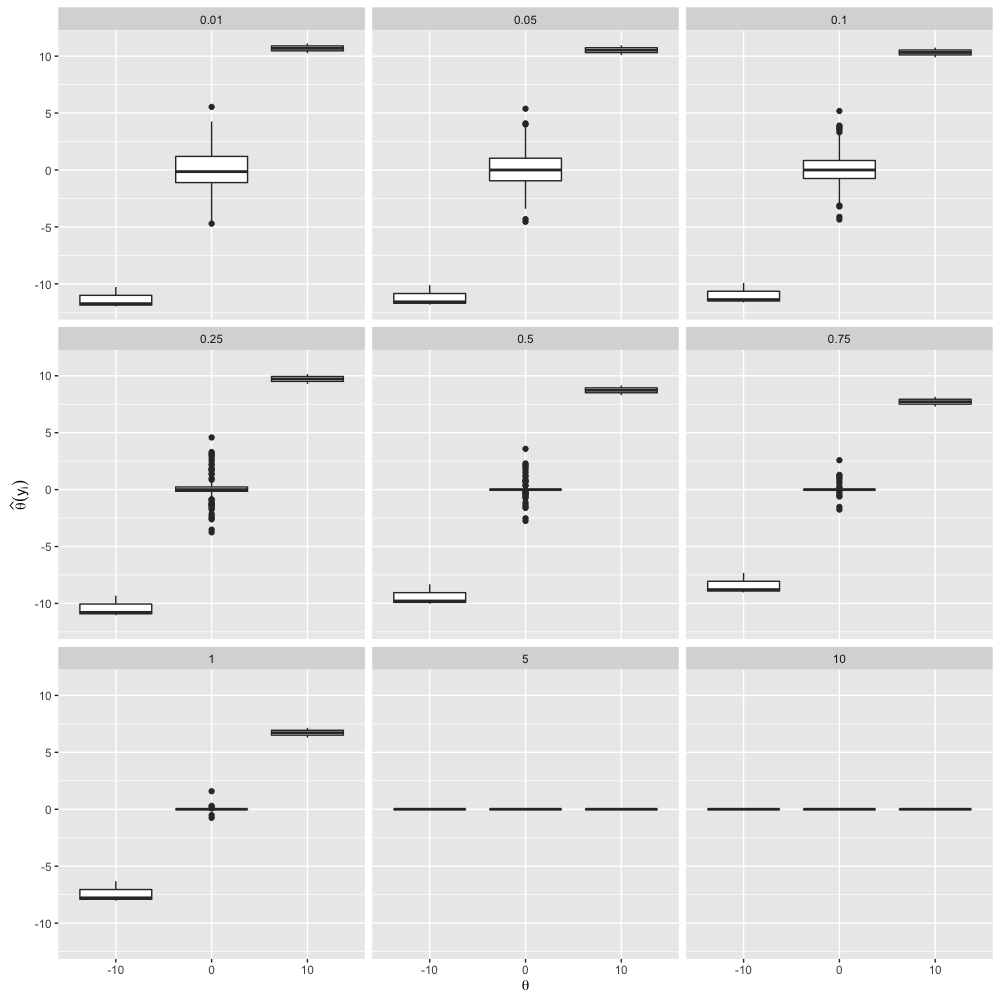
\includegraphics[scale=0.5]{sparsity.png}

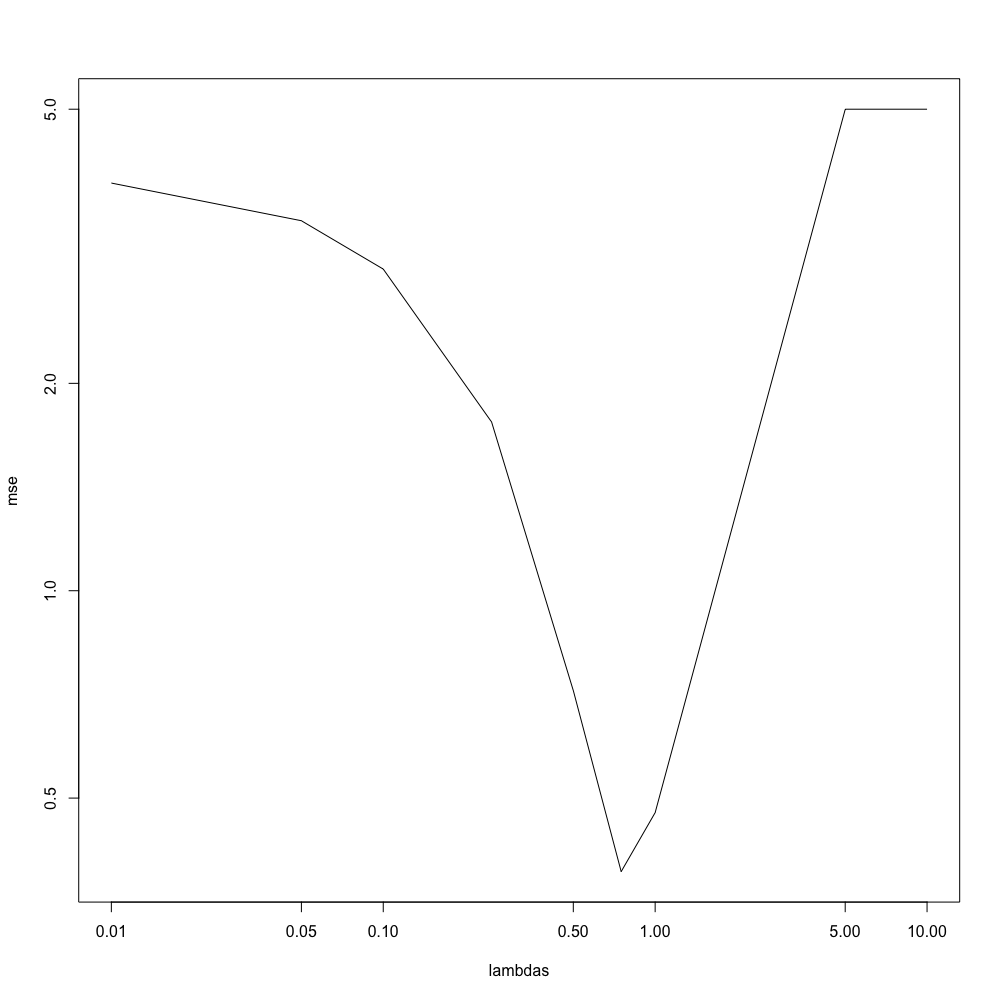
\includegraphics[scale=0.5]{mse_lambdas.png}

\subsubsection{Notes from class}
This independent normal means toy problem is useful for orthogonal decompositions for Fourier analysis or wavelets.
The context of wavelets is:
\begin{align*}
y_i&=f(x_i)+e_i\\
f(x)*=\sum_{k=1}^D \theta_k \psi_k(x)
\end{align*}
where $\psi_k$ are basis functions and $\theta_k$ are coefficients. $\psi_k$ in wavelets are generally not closed-form, but
easy to graph (see Haar and Daubechies). This reduces down to a regression of normal means (especially if you have $n=2^d$ observations for some $d$, then split the Haar basis functions $d$ times and get $2^d$ values, that means
that you get $D=2^d$ and you don't want overfitting, so you're just fitting the $\theta_k$ by shrinking normal means.


\section{The lasso}

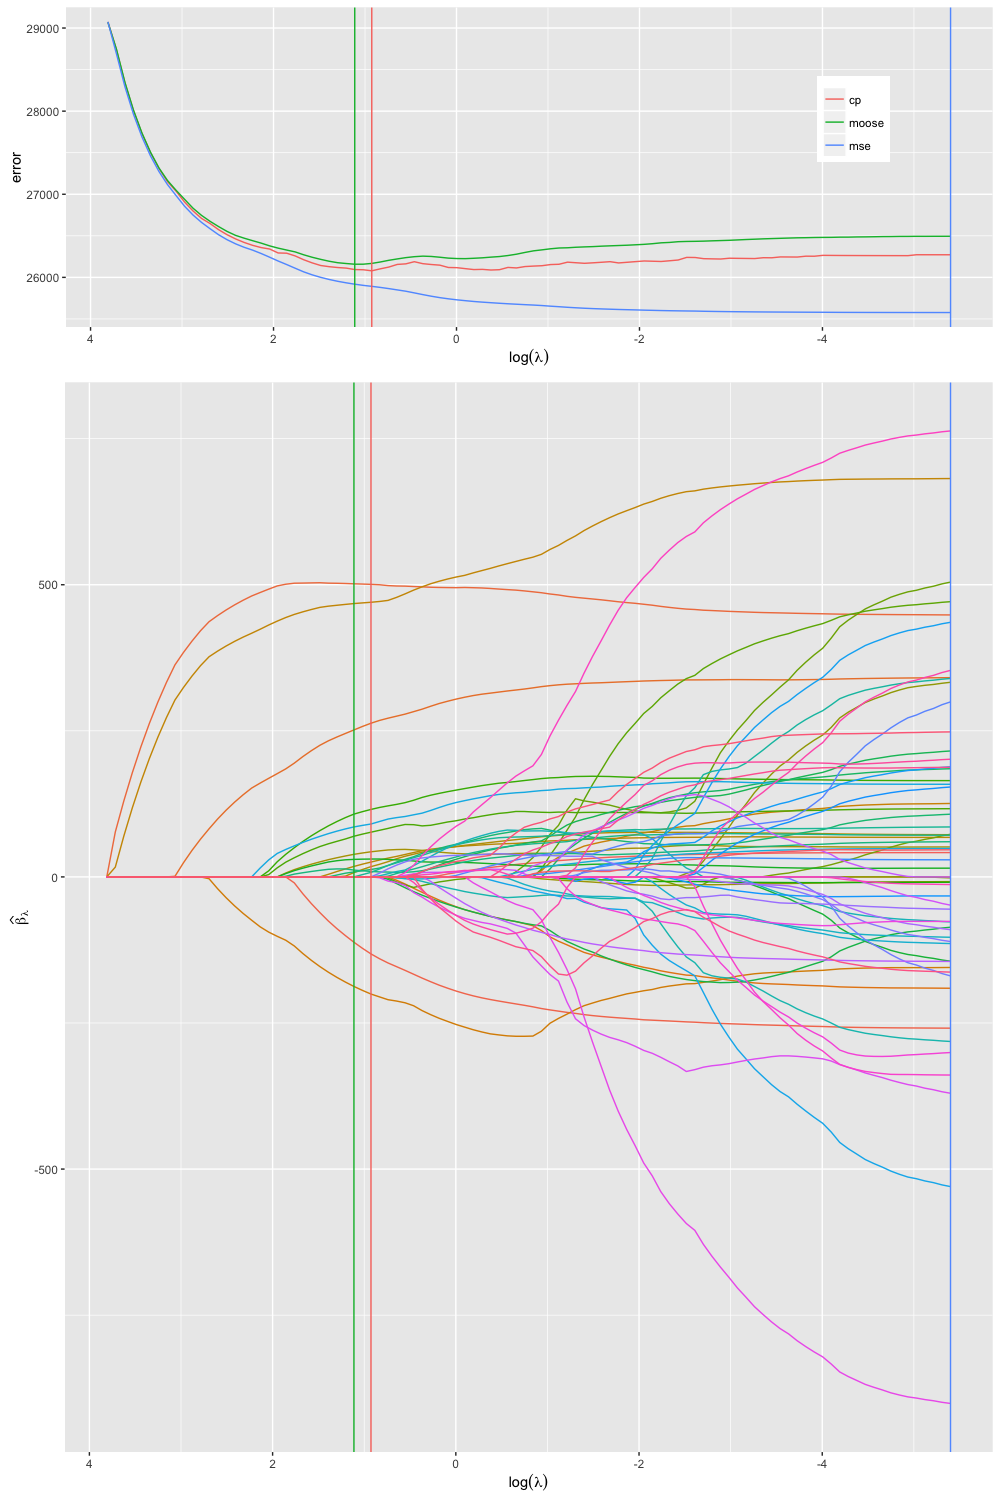
\includegraphics[scale=0.35]{overall.png}

\end{document}